% ============================================================
% 正文：Research Methodology
% 作者：Kehui Chen, Jacky Keung, Xiaoxue Ma
% 主题：MCP 故障定位（fault localization）根因实证研究
% ============================================================

\section{Research Methodology}\label{sec:method}

We adopt a sequential-exploratory mixed-methods design combining qualitative and
quantitative evidence \cite{ostlund2011combining}. The overview is shown in Fig.~\ref{fig:methodology}.

The design has two phases. \textbf{Phase 1 (demand side):} semi-structured interviews with
MCP practitioners capture the perceived pain points of MCP adoption, with particular focus
on fault diagnosis. \textbf{Phase 2 (technical side):} guided by these pain points, we mine a
real-bug dataset from the official MCP SDK issue tracker, reproduce a subset at runtime, and
run observability experiments to quantify the technical root causes. The two phases are
triangulated: interview findings motivate the experimental design, and experimental results
objectively verify the interview complaints.

\noindent
\begin{minipage}{\linewidth}
  \centering
  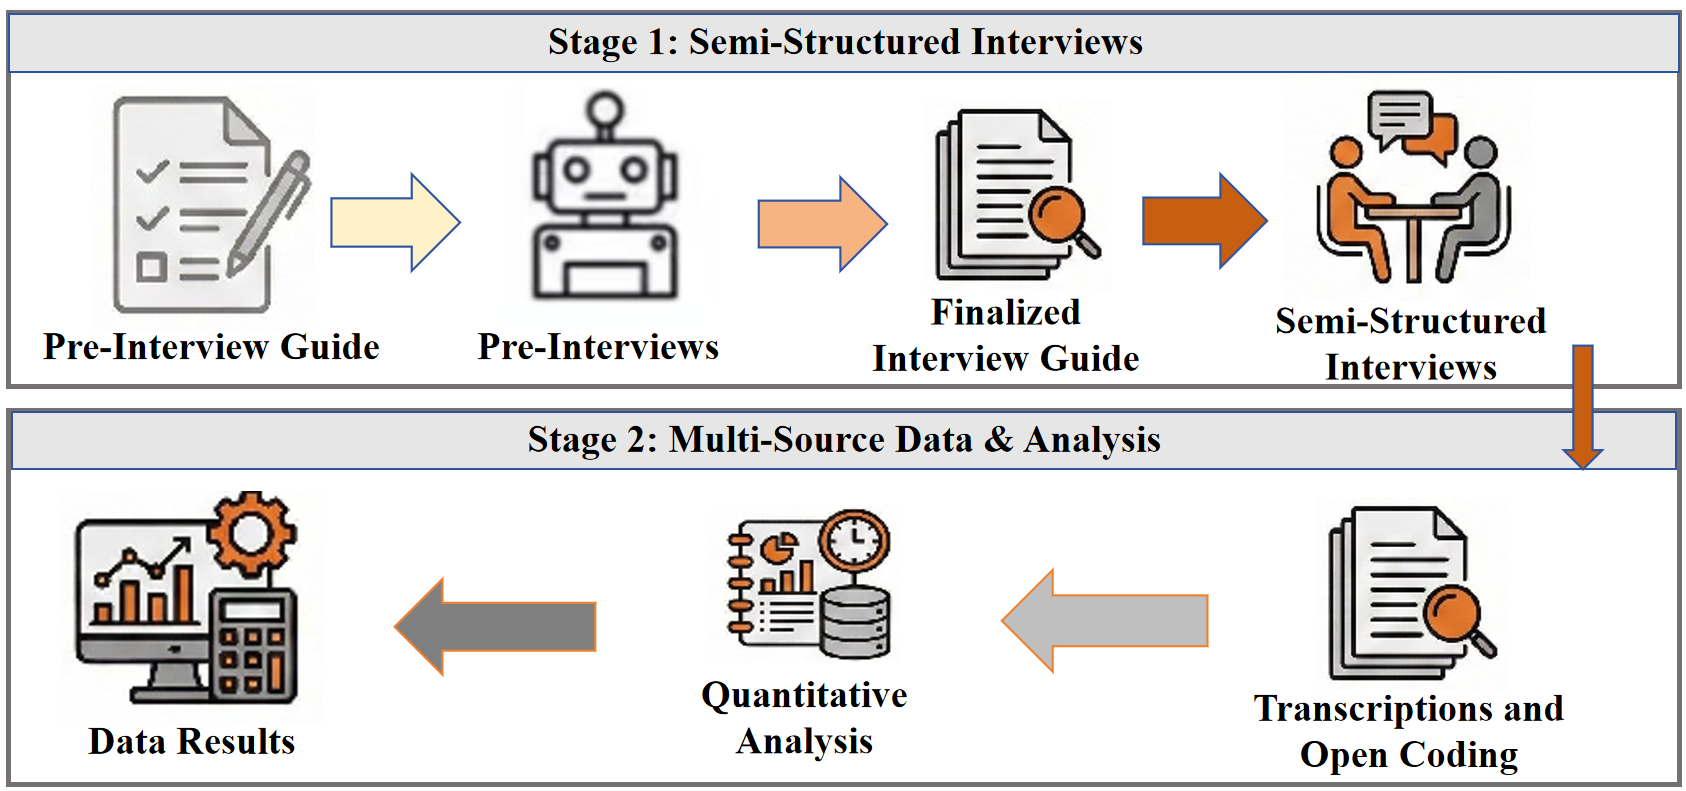
\includegraphics[width=\linewidth]{figs/methodology}
  \captionof{figure}{Overview of the sequential-exploratory mixed-methods methodology.}
  \label{fig:methodology}
\end{minipage}

\subsection{Phase 1: Semi-Structured Interviews}

We use expert sampling, a subtype of purposive sampling \cite{baltes2022sampling}, and
conduct semi-structured interviews with 20 practitioners in the MCP field, preceded by three
pre-interviews to refine the interview guide \cite{adeoye2021research}.

\textbf{Interview design.} We drafted initial questions from the literature
\cite{ma2025practitioners} and revised them through pre-interviews. The final guide contains
open-ended questions \cite{le2014loaded}; participants could answer ``I don't know'' to reduce
response bias. We finalised 31 core questions covering demographics, MCP practices and
problems, technical capability assessment, security and privacy, future expectations, and
counterintuitive insights.

\textbf{Procedure.} We conducted pre-interviews with three participants; formal interviews
were held online, each lasting 90--120 minutes, and were transcribed verbatim (~400,000 words
of original data). We conducted secondary interviews with ten key participants (30 minutes
each) to clarify vague views. Sample size was determined by theoretical saturation: no new
viewpoints appeared after 20 interviews \cite{ma2025practitioners}.

\textbf{Participants.} We recruited 20 MCP practitioners from FinTech and Internet industries
(e.g., HSBC, Huawei); 9 from FinTech and 11 from Internet. Participants cover all core MCP
roles (Host, Client, Server, User) and multiple job roles (Senior Architect, Software
Developer, Business Analyst, Algorithm Designer), as summarised in
Table~\ref{tab:participants}. Experience ranges from 2 to 20 years; team sizes range from 6
to 160 people.

\begin{table}[!t]
\centering
\caption{Participant demographics and experience distribution.}
\label{tab:participants}
\scriptsize
\renewcommand{\arraystretch}{1.05}
\setlength{\tabcolsep}{1.6pt}
\begin{tabular}{@{}c c c c c c c@{}}
\toprule
\textbf{ID} & \textbf{Role} & \textbf{Ind.} & \textbf{MCP} & \textbf{Mgmt.} & \textbf{Exp.} & \textbf{Team} \\
\midrule
P1  & SA & F & H/C/S & Y & $>$10 & $>$80 \\
P2  & SA & I & H/C/S & Y & $>$10 & $>$80 \\
P3  & SA & I & H/C/S & Y & $>$10 & $>$80 \\
P4  & SA & I & H/C/S & Y & 3--10 & 21--40 \\
P5  & SD & F & C/S   & N & 3--10 & 21--40 \\
P6  & SD & I & C/S   & N & 3--10 & 21--40 \\
P7  & SD & F & C/S   & N & 3--10 & 21--40 \\
P8  & SD & I & C/S   & N & 3--10 & 21--40 \\
P9  & SD & F & C/S   & N & 3--10 & 21--40 \\
P10 & SD & I & C/S   & N & 3--10 & 21--40 \\
P11 & SD & F & C/S   & N & 3--10 & 41--80 \\
P12 & SD & I & C/S   & N & 3--10 & 41--80 \\
P13 & SD & F & S     & N & 3--10 & 41--80 \\
P14 & SD & I & S     & N & $<$3 & 41--80 \\
P15 & BA & F & U     & N & 3--10 & 21--40 \\
P16 & BA & I & U     & N & 3--10 & 21--40 \\
P17 & BA & F & U     & N & 3--10 & 21--40 \\
P18 & BA & I & U     & N & 3--10 & 41--80 \\
P19 & AD & F & S     & Y & 3--10 & 21--40 \\
P20 & AD & I & S     & Y & $>$10 & $>$80 \\
\bottomrule
\end{tabular}
\vspace{0.35em}
\parbox{\columnwidth}{\scriptsize\raggedright
\textit{Note:} SA = Senior Architect; SD = Software Developer; BA = Business Analyst; AD = Algorithm Designer; F = FinTech; I = Internet; H/C/S = Host/Client/Server; C/S = Client/Server; S = Server; U = User; Y/N = management responsibility. Experience is reported in years.}
\end{table}

\subsection{Phase 2: Real-Bug Dataset and Observability Experiments}

Guided by the demand-side evidence, we build a real-bug dataset by mining the entire issue
tracker of the official \verb|modelcontextprotocol/python-sdk|, reproduce a representative
subset at runtime over the production Streamable-HTTP transport, and run observability
experiments that quantify the technical root causes of fault-localisation difficulty. The
dataset construction, the four-layer taxonomy, and the experiment configuration are described
in detail in Section~\ref{sec:setup}.

\subsection{Definition of the Four-Layer Fault Taxonomy}\label{sec:taxonomy}

The MCP protocol itself defines four components: the Host, the Client, the Server, and the
Resource (the data / context that the Server exposes) \cite{yang2025survey}. Because a Resource is
a piece of exposed data rather than a process that can malfunction on its own, faults involving a
Resource are ultimately triggered by one of the other three components (e.g.\ a Host or Client
supplying a wrong resource identifier, or a Server mishandling it). We therefore classify a fault
by the component or the transport link in which it actually originates, giving four layers covering
the three components (Host, Client, and Server) together with the transport between them. Faults may
arise in any of the three components or during the transport of the messages between them, so we
classify a fault by the layer in which it originates:

\begin{itemize}
  \item \textbf{Host scheduling layer (H):} faults originate from the Host/LLM caller,
        such as invoking a non-existent tool, missing or mis-spelled arguments, and wrong
        argument types.
  \item \textbf{Client message layer (C):} faults caused by malformed JSON-RPC request
        payloads assembled on the Client side, such as redundant parameters, incorrect
        argument nesting, and invalid enumeration values.
  \item \textbf{Server tool layer (S):} faults occurring inside the execution logic of MCP
        Server tools, such as division-by-zero, index-out-of-range, assertion failures,
        custom business exceptions, oversized responses, duplicate tool registration, and
        permission-denied errors.
  \item \textbf{Transport layer (T):} session-level and message-passing faults, including
        calling tools after session closure, cancelled in-flight requests, invalid raw
        protocol messages, and invoking methods before session initialisation.
\end{itemize}

\subsection{Data Analysis}

We transcribed the interview content verbatim and used open coding \cite{ma2025practitioners}
to generate an initial code set. The first two authors conducted cross-validation of the
coding logic; Cohen's kappa reached 0.89 (high consistency), and disagreements were resolved
by consensus. We extracted the core issues related to fault diagnosis (the core obstacles to
MCP deployment) and the expected improvements (the solutions practitioners desire).
Quantitative analysis \cite{nevin1984quantitative}
was applied to quantifiable content, complemented by qualitative analysis for open-ended,
exploratory responses.